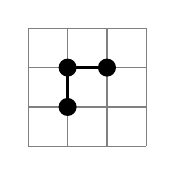
\begin{tikzpicture}
	%grid
	\draw [black!50,step=0.5] (0, 0) grid (1.5, 1.5);

	%nodes
	\foreach \p in {
		(0.5, 0.5),
		(0.5, 1),
		(1.0, 1)
	}\draw [thick, fill=black] \p circle (0.1);

	%paths
	\draw [very thick, color=black] plot coordinates {
		(0.5, 0.5)
		(0.5, 1)
		(1.0, 1)
	};

\end{tikzpicture}
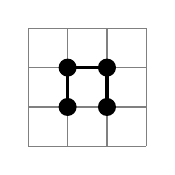
\begin{tikzpicture}
	%grid
	\draw [black!50,step=0.5] (0, 0) grid (1.5, 1.5);

	%nodes
	\foreach \p in {
		(0.5, 0.5),
		(0.5, 1),
		(1.0, 1),
		(1.0, 0.5)
	}\draw [thick, fill=black] \p circle (0.1);

	%paths
	\draw [very thick, color=black] plot coordinates {
		(0.5, 0.5)
		(0.5, 1)
		(1.0, 1)
		(1.0, 0.5)
	};

\end{tikzpicture}
